% !Mode:: "TeX:UTF-8"
%!TEX program  = xelatex

%本模板借用数模竞赛模板
%模板名称:YangThesis

%去掉封面,withoutpreface选项
%\documentclass[no-math,withoutpreface,bwprint]{YangThesis} 

%采用封面
\documentclass[no-math,bwprint]{YangThesis} 

%导入设置文件
%设置参数均存储在settings.tex文件中,
%添加或修改需要在该文件中进行
% settings.tex
% YangTemplate.cls 的配置文件
% 采用<\input>放入主文档中,不可单独编译

\usepackage[T1]{fontenc}

% 正文和数学字体均采用Times New Roman字体
% \usepackage{newtxtext, newtxmath}

% 只正文采用Times字体,数学公式保持默认字体
\usepackage{newtxtext}

\usepackage{float}

% 定制tikz流程图形状
\usepackage{tikz}
\usetikzlibrary{shapes.geometric, arrows}
% 开始
\tikzstyle{startstop} = [rectangle, rounded corners, minimum width = 2cm, minimum height=1cm,text centered, draw = black]
% 输入输出
\tikzstyle{io} = [trapezium, trapezium left angle=70, trapezium right angle=110, minimum width=2cm, minimum height=1cm, text centered, draw=black]
% 过程
\tikzstyle{process} = [rectangle, minimum width=3cm, minimum height=1cm, text centered, draw=black]
% 判断
\tikzstyle{decision} = [diamond, aspect = 3, text centered, draw=black]
% 箭头形式
\tikzstyle{arrow} = [->,>=stealth]

% 设置编号格式
\newcounter{rowno}
\numberwithin{equation}{section}
\numberwithin{figure}{section}
\numberwithin{table}{section}
\renewcommand{\thefigure}{\arabic{section}-\arabic{figure}}
\renewcommand{\thetable}{\arabic{section}-\arabic{table}}
\renewcommand{\theequation}{\arabic{section}-\arabic{equation}}

% 新数学命令
\newcommand\dif{\mathrm{d}}
\newcommand\no{\noindent}
\newcommand\dis{\displaystyle}
\newcommand\ls{\leqslant}
\newcommand\gs{\geqslant}

\newcommand\limit{\dis\lim\limits}
\newcommand\limn{\dis\lim\limits_{n\to\infty}}
\newcommand\limxz{\dis\lim\limits_{x\to0}}
\newcommand\limxi{\dis\lim\limits_{x\to\infty}}
\newcommand\limxpi{\dis\lim\limits_{x\to+\infty}}
\newcommand\limxni{\dis\lim\limits_{x\to-\infty}}

% 默认上限为无穷
\newcommand\sumnf{\dis\sum\limits_{n=1}^{\infty}}
\newcommand\sumnz{\dis\sum\limits_{n=0}^{\infty}}
\newcommand\sumkf{\dis\sum\limits_{k=1}^{\infty}}
\newcommand\sumkz{\dis\sum\limits_{k=0}^{\infty}}
\newcommand\sumifn{\dis\sum\limits_{i=1}^{n}}
\newcommand\sumizn{\dis\sum\limits_{i=0}^{n}}
\newcommand\sumkzn{\dis\sum\limits_{k=0}^n}
\newcommand\sumkfn{\dis\sum\limits_{k=1}^n}

\newcommand\pzx{\dis\frac{\partial z}{\partial x}}
\newcommand\pzy{\dis\frac{\partial z}{\partial y}}

\newcommand\pfx{\dis\frac{\partial f}{\partial x}}
\newcommand\pfy{\dis\frac{\partial f}{\partial x}}

\newcommand\pzxx{\dis\frac{\partial^2 z}{\partial x^2}}
\newcommand\pzxy{\dis\frac{\partial^2 z}{\partial x\partial y}}
\newcommand\pzyx{\dis\frac{\partial^2 z}{\partial y\partial x}}
\newcommand\pzyy{\dis\frac{\partial^2 z}{\partial y^2}}

\newcommand\pfxx{\dis\frac{\partial^2 f}{\partial x^2}}
\newcommand\pfxy{\dis\frac{\partial^2 f}{\partial x\partial y}}
\newcommand\pfyx{\dis\frac{\partial^2 f}{\partial y\partial x}}
\newcommand\pfyy{\dis\frac{\partial^2 f}{\partial y^2}}

\newcommand\intzi{\dis\int_{0}^{+\infty}}
\newcommand\intd{\dis\int}
\newcommand\intab{\dis\int_a^b}

\newcommand\mc{\mathbb{C}}
\newcommand\mr{\mathbb{R}}
\newcommand{\degree}{^\circ}

\newenvironment{mfrac}[2]%
{\raise0.5ex\hbox{$#1$}\! \left/ \! \lower0.5ex\hbox{$#2$}\right.}

% 定义新数学符号
\DeclareMathOperator{\sgn}{sgn}
\DeclareMathOperator{\arccot}{arccot}
\DeclareMathOperator{\arccosh}{arccosh}
\DeclareMathOperator{\arcsinh}{arcsinh}
\DeclareMathOperator{\arctanh}{arctanh}
\DeclareMathOperator{\arccoth}{arccoth}
\DeclareMathOperator{\grad}{\bf{grad}}
\DeclareMathOperator{\diag}{diag}
\DeclareMathOperator{\csign}{csign}

\usepackage{url}

% 自定义字号大小命令
% 修改18pt为想要的字号即可
\newcommand{\myfont}{\fontsize{18pt}{\baselineskip}\selectfont}

% 参考文献标号为上标
\newcommand{\upcite}[1]{\textsuperscript{\textsuperscript{\cite{#1}}}}

% 定制页眉页脚
\usepackage{fancyhdr}
\pagestyle{fancy}
% 页眉
\lhead{}
\chead{基于神经网络的机器人智能抓取研究}
\rhead{}
% 页脚
\lfoot{}
\cfoot{-\thepage-}
\rfoot{}

% 页眉页脚单横线
%\renewcommand{\headrulewidth}{0.4pt}
%\renewcommand{\footrulewidth}{0pt}

% 页眉双横线
\newcommand{\makeheadrule}{%
\makebox[0pt][l]{\rule[0.2\baselineskip]{\headwidth}{1.3pt}}%
\rule[0.35\baselineskip]{\headwidth}{2.5pt}}
\renewcommand{\headrule}{%
{\if@fancyplain\let\headrulewidth\plainheadrulewidth\fi
\makeheadrule}}
\makeatother

% 设置脚注编号格式
\renewcommand{\thefootnote}{\fnsymbol{footnote}}



% 封面信息
\papercategory{人工智能课程论文}
\title{基于神经网络的机器人智能抓取研究}
\schoolname{哈尔滨工业大学(深圳)}
\departname{机电工程与自动化学院}
\classnumber{机械二班}
\authorname{杨敬轩}
\studentID{SZ160310217}
\dateinput{2019年04月10日}

%开始写文章
\begin{document}

%生成标题
 \maketitle

 %页码从1开始计数
 \setcounter{page}{1}
 %页码采用罗马数字格式
 \pagenumbering{Roman}
 
 %若有封面,以下可删=========================
 \vspace{0.5cm}
 \hfill{——杨敬轩\footnote{\small 哈尔滨工业大学(深圳),
 机电工程与自动化学院,机械类专业}}\par
 \hfill{——SZ160310217}
 %%=======================================
 
 %开始写摘要
 \begin{abstract}
 %将摘要添加到目录中
 \addcontentsline{toc}{section}{摘要}
 
本文针对不同加工情况下智能RGV动态调动问题,构建了基于最短路径贪心算法、及改良的模拟退火算法的动态调度模型,运用了 MATLAB编程求解以及FlexSim模拟加工过程,给出针对一道工序,两道工序以及考虑故障情况时一道工序和两道工序四种RGV动态调度方案,以及两道工序下分配8台CNC装配不同加工刀具排布的方案,并给出以绝对理想情况为比较依据的系统的作业效率。

%关键词
\keywords{模拟退火算法;贪心算法;最短路径;RGV;动态调度;作业效率}
\end{abstract}

%强制目录二字位于最上方
\vspace{-1.3cm}
%生成目录
\tableofcontents
%将目录项添加到目录中
\addcontentsline{toc}{section}{目录}

%撰写正文
\clearpage
%调整标题与上边的距离
\vspace{-1cm}
%第1章的标题
\section{研究背景}

%页码从1开始计数
\setcounter{page}{1}
%页码格式采用阿拉伯数字
\pagenumbering{arabic}

%正文内容,注意LaTeX分段由两种方法,直接空一行或者使用\par
%默认首行缩进,不需要在这里手动敲空格,已有宏包处理
随着社会发展,人口老龄化,劳动力短缺等问题逐渐凸显,对服务机器人的需求也越来越大,但是服务机器人所工作的非结构化环境也带来了许多技术难题,其中十分主要的一个问题就是非结构环境中机器人的自动抓取,因为抓取是机器人与现实世界交互的主要方式之一。不同于工业机器人在结构化环境中对工件的抓取,服务机器人在非结构化环境下的自动抓取面临着诸多挑战,例如动态化环境、光照变化、物体间存在相互遮挡,以及最主要的,非结构化环境中除了已知的物体,还有大量未知物体,而多数工业机器人上应用十分成熟的抓取规划方法依赖于预先获取物体的模型来建立数据库,而对于非结构化环境中工作的服务机器人,预先获取所有需要进行抓取的物体的模型是不现实的,因此机器人必须能够对未知的物体在线进行快速稳定可靠的抓取规划。

为了解决上述问题,常用的一种做法就是使用机器学习方法来学习从传感器数据提取出的特征表达到抓取位姿的映射关系,相比于建立物体的模型库来保存抓取经验,机器学习方法可以在没见过的物体上进行抓取经验的迁移。在这个领域中,一些传统的方法通常借助于人工设计的特征来表示和存储抓取经验,并训练分类器,但人工设计的特征往往只针对于某一种特定物体或任务有效,且人工设计特征的工作量大难度高,很难在其他场景进行使用。
 
近年来,以卷积神经网络(Convolutional Neural Network, CNN)为代表的深度学习技术,在计算机视觉,自然语言处理,语音,医疗,机械设备健康监测等诸多领域取得了重大的突破,在一些领域中达到了超过人类的性能。卷积神经网络已经在许多机器人相关的研究领域得到了应用,比如被广泛地应用于目标识别,目标检测,目标跟踪,图像语义分割,即时定位与建图等。相比于繁琐复杂的人工特征设计,卷积神经网络可以通过大量数据的训练挖掘出适合于当前任务的特征表达,由于通常卷积神经网络需要堆叠很多层来提高特征表达能力,因此参数较多,需要使用比传统机器学习算法更多的标注数据来进行训练,抑制过拟合提高算法的泛化能力。但随着互联网大数据时代的到来,训练数据的获取变得比以前更加容易,因此卷积神经网络研究不断取得突破。

在机器人抓取规划领域,使用卷积神经网络学习的特征取代人工设计的特征来对抓取进行表示和分类有很大的优势和应用前景。首先,相比于人工设计的特征,卷积神经网络通过大量数据的学习可以挖掘出泛化能力更强效果更好的特征,可以进一步提高抓取规划算法的性能,且省去了复杂的人工特征设计工作。其次,随着硬件计算力和仿真软件性能的提升,视觉传感器的普及,目前已有许多通过实验或者仿真收集的机器人抓取数据集可供使用。
 
综上,有了足够的数据以及合理设计的卷积神经网络结构就可以建立更高性能的自动抓取规划算法,进而提高服务机器人在非结构化环境的交互能力,提高其自主化和智能化程度,提高服务机器人的实用性和推进产业落地。因此,基于卷积神经网络的机器人自动抓取规划具有重要的研究价值,可以带来巨大的经济效益。

%需手动分页,为实现分页与不分页均可
\newpage
\section{文献综述}

\subsection{抓取物体图像识别}

近年来,基于深度学习的方法已经在包括视觉识别\cite{bib1,bib2},语音识别和自然语言处理等任务上取得了重大成就。美国康奈尔大学 Lenz 等\cite{bib3}借鉴深度学习在图像检测及图像识别等任务中的成功经验,提出了基于深度学习的机器人抓取检测的方法\cite{bib3,bib4}。与传统的依靠人工经验抽取样本点特征的方式相比,基于深度学习的机器人抓取检测的方法可以自动学习如何识别和提取待抓取位置的特定特征。越来越多的机器人学者研究如何将深度学习的方法应用于机器人抓取检测上从而使机器人具备更强大的智能。大部分研究学者都是将深度学习的方法用来学习不同形状和位姿的物体的末端执行器的最佳配置,基于深度学习的深层表达能力学习的参数为每个图像预测多个抓取位置进行排序来找到最佳抓取位置。

基于深度学习的方法,Lenz 等\cite{bib3}提出了基于稀疏自编码器的两步级联抓取检测系统,构建两个大小网络用于提取 RGB-D 输入数据的抓取特征,采用滑动窗的方法搜索抓取框,最后在网络顶层添加支持向量机(Support Vector Machine,SVM)作为分类器的网络结构。在标准康奈尔抓取数据集\cite{bib6}上达到 73.9\%的检测准确率,耗时13.5s,由于采用类似于穷举法的搜索机制,需要在不同大小的图像块上使用分类器进行重复计算,计算量非常大,且十分耗时。

Redmon 等\cite{bib7}认为采用滑动窗口的方法来预测抓取位置是一种非常耗时的方法,而且使用单阶段的网络性能优于 Lenz 等的级联系统。为了避免在不同大小的图像块上重复计算,他们利用卷积神经网络强大的特征提取能力将整个图像输入网络中,在整个图像上直接进行全局的抓取预测,目前大部分学者采用这种方案\cite{bib5,bib8}。使用类似于 AlexNet\cite{bib9}的卷积神经网络模型来实现单阶段的检测方法,以更快的速度达到了更高的检测精度,但是这种方法由于卷积神经网络结构的复杂性仍然存在模型较大的缺陷。 

Kumra 等\cite{bib4}也采用将整个图像输入卷积神经网络中进行全局的抓取预测,网络结构上,他们采用网络结构更复杂特征提取能力更强的ResNet50\cite{bib10}提取抓取特征,用 SVM 预测抓取配置的参数。精度上可以达到比较好的检测精度,但是由于模型采用层数较深的残差网络,导致网络模型和计算量都比较大。

Chu 等\cite{bib5}提出了一种适合于多物体场景抓取模型,首先使用 ResNet50 对输入图像提取抓取特征,然后使用类似于 RPN  网络的模型进行抓取框的推荐,最后经 ROI  Pooling 进行角度参数的分类和抓取框的回归。这种模型适用于多物体的抓取场景, 并且达到了较高的抓取检测准确率,由于模型较深且类似于级联系统导致模型较大。
 
综上所述,目前基于神经网络的机器人抓取位姿预测方法的研究主要集中在结合基础分类网络 如 AlexNet、ResNet 等提高抓取检测准确性上,这些网络最初是为复杂的分类任务和海量数据的特点而设计的,网络结构通常具有大量的参数,需要大量的计算和存储资源。针对上述深度学习抓取检 测方法的不足,本文提出了基于 SqueezeNet 的轻量级卷积神经网络抓取预测模型,在不降低准确率的情况下,本文提出的网络模型更小,需要的存储资源更少,速度更快,更适合于移动机器人平台中。 类似的设计轻量级模型的工作如\cite{bib11}。

\subsection{机器人抓取策略}
在机器人分拣、 搬运等抓取作业任务中,包括顶抓(top-grasp)和侧抓(side-grasp)2 种方式的平面抓取(planar grasp)是最为常用的抓取策略。对于任意姿态的未知不规则物体,在光照不均、 背景复杂的场景下,如何利用低成本的单目相机实现快速可靠的机器人自主抓取姿态检测具有很大的挑战。

机器人自主抓取姿态规划方法根据感知信息的不同可分为 2 类:一类是基于物体模型的抓取姿态估计 \cite{bibb1,bibb2,bibb3},一类是不依赖物体模型的抓取姿态检测。基于模型的方法需要给定精确、 完整的物体 3 维模型,然而低成本相机的成像噪声大,很难扫描建立精确模型。另外,基于 3 维模型的方法计算复杂,难以适应机器人实时抓取判断的需求。

不依赖物体模型的方法借助于机器学习技术,其实质是将抓取位姿检测问题转化成目标识别问题。例如,文 \cite{bibb4} 提出了一种用 2 维矢量矩形表示图像上物体抓取位姿的直观方法。机器学习方法的出现令抓取检测不局限于已知物体。早期的学习方法 \cite{bibb4} 需要人为针对特定物体设定特定的视觉特征,不具备灵活性。近年来,深度学习 \cite{bibb5} 发展迅速,其优越性正在于可自主提取与抓取位姿有关的特征。 

机器人抓取检测问题包括 2 个部分:抓取位置确定和抓取姿态估计。传统的位置检测方法根据二值化的图像计算物体重心作为抓取位置,但是可抓取位置不在重心处的物体甚多。通常采用滑动窗口法\cite{bibb6,bibb7} 解决抓取点不在重心上的问题,但此方法以遍历搜索获得最优解,时间代价大。文\cite{bibb8} 对此作出了改进,通过缩小搜索区域范围并减少搜索窗旋转次数来实现时间的优化。Pinto 等人\cite{bibb9}尝试用随机采样法缩短定位时间,但检测结果因依赖采样位置而表现不稳定,且计算时间减少的成效不明显。 在抓取姿态估计方面,文\cite{bibb7,bibb10}将最优搜索窗的旋转角度作为抓取角度,文\cite{bibb9} 率先以旋转角度为标签将抓取检测感知部分当作分类问题解决,但这些属于粗估计方法,低精度的抓取角度可导致机器人在实际抓取时因受力点错误而抓取失败。因此,减少抓取定位时间消耗和提升姿态估计精度是机器人在线抓取检测时亟待解决的 2 个问题。

深度神经网络用于机器人抓取位姿检测的另一个问题是,已有公开模型如文\cite{bibb7}和文\cite{bibb11}所提出的模型等都是在封闭大数据集上训练所得,通常需要随机器人部署而扩展关于实际特定抓取对象的小样本数据集。迁移学习为特定任务小样本集下深度网络模型训练提供了方法。自建的数据集规模虽小,但能够在已经过百万级封闭数据集训练并具有基本特征提取能力的模型上微调训练,令在特定小样本集下训练的模型仍具有卓越的性能。这样不仅能缩短训练周期,还可提升整个系统的拓展性。

本文针对任意姿态的未知不规则物体,提出一种适于顶抓策略的平面抓取位姿快速检测方法。本文主要研究内容及贡献包括:

1) 提出一种抓取姿态细估计的卷积神经网络模型 Anlge-Net。

2) 在此基础上,提出一种两阶段级联式抓取位姿检测模型。模型第 1 阶段先以基于区域的全卷积网络\cite{bibb12}为基础提取少量且可靠的候选抓取位置, 再对候选结果筛选排序确定最优抓取位置,以此加快检测速度;第 2 阶段为 Angle-Net 在前一阶段输出的局部位置图像下计算抓取角度。 相比于文\cite{bibb9}的方法,直接计算的抓取角度误差更小,抓取检测精度得以提升。

3) 模型训练过程中使用了迁移学习\cite{bibb13}机制,在保证数据集可动态扩展的同时又缩短了训练周期。

4) 在公开数据集和实际场景下进行抓取检测方法效果验证。实验证明,该抓取检测方法速度快(17.5 帧/秒),准确率高,鲁棒性强。

\newpage
\section{典型神经网络案例分析}

\subsection{基于复值神经网络的机器人抓取}

\subsubsection{实值神经网络发展历程}

人类利用人工神经网络对生物神经网络的结构、机理和功能模拟的研究,经历了近半
个多世纪漫长而又曲折的过程。具有里程碑意义的是如下三个模型\cite{bibc1,bibc2}.

1943年神经生理学家McCulloch和数学家Pitts提出的第一个人工神经网络模型:
McCulloch-Pitts模型\cite{bibc3},成为神经网络研究的开端。1949年心理学家D.O.Hebb在文献\cite{bibc4}中提出了神经元之间突触联系强度可以改变的假设,并据此提出了神经元学习的准则,为神经网络的学习算法奠定了基础。这些重大进展促进了神经网络早期的研究。

1958年Rosenblat将McCulloch和Pitts的工作与Hebb的工作结合在一起,设计出的
一种称为感知机的神经网络模型\cite{bibc5},首次把人工神经网络的研究从理论付诸工程实践,引起了许多科学家的兴趣。不过在1969年,人工智能创始人之一Minsky和Papert出版了以《感知机》为名的书\cite{bibc6},书中从数学上深入分析了感知机的原理,指出了其局限性并从理论上对感知机的原理给予了沉重的打击,使得神经网络早期的研究热潮迅速降温,并开始陷入低潮和休眠状态。

1982年和1984年美国加州理工大学的生物物理学家J.J.Hopfield提出了Hopfield神经
网络\cite{bibc7,bibc8}。Hopfield神经网络模型的提出具有划时代的伟大意义,使得神经网络的研究从体眠的状态开始复苏。Hopfield在文献\cite{bibc7,bibc8}中设计出用电子电路实现这一网络的方案,从而为神经计算机的研究奠定了基础。更为重要的是他把设计出的神经网络应用于联想记忆以及解决优化领域一直困扰的TSP问题,并取得了巨大的成功,这些重大进展大大促进了神经网络的研究。此外,他还通过引入类似于Lapunov函的“计算能量函数”的概念对网络的动力学特性进行了分析并给出了网络稳定性的条件,从而开启了神经网络稳定性研究。

\subsubsection{复值神经网络的兴起}

复值神经网络(Complex-valued Neural Network)是实值神经网络在复数域的推广。相比实值神经网络,复值神经网络的起步稍晚。其历史可追溯到1975年Widrow提出的复值最小均方(LMS)算法,该算法后来被广泛运用于信号处理领域\cite{bibc9}。但正如复数的出现和被人认可经历了一个漫长的过程一样,复值神经网络在出现后的相当长时间,并未引起人们的重视。直至近几年来,随着神经网络应用领域的不断扩展,许多需要处理复数信号的领域也提出了用神经网络解决其相关问题的要求,例如量子力学、电磁学、光电子、图像、遥感、时间序列分析等。在这些领域中,基于复数信号的表示、分析和处理具有极大的便利,而复值神经网络则能直接处理复数信号,因而很自然地使二者联系在一起。事实上,在需要幅值和相位(或理解为大小和方向)两方面信息来表示同一信号的场合,运用复值神经网络较之实值神经网络,要更为直接。尽管可以用2个实值神经网络分别表达此类信号的大小和方向(或实部和虚部),但正如复数虽然只是两个实数按某种规则而连接,但依然有其独立于实数而存在的必要性一样,复值神经网络由于复数有实部和虚部,且复数运算规则的特殊性等原因,在其实现和运用过程中表现出一些实值神经网络所不具有特质,因此复值神经网络也不能简单地理解为可用2个实值神经网络所取代。而且在将神经网络从实数域到复数域的推广中,并不是像表面上理解的那样:仅是简单地将一个变量从实数变成复数。如果这样做的话,许多诸如奇异等意想不到的问题就有可能发生\cite{bibc10}。

作为复值神经网络研究领域的先导者,日本的Akira Hirose教授总结了近年来复值神经网络的研究成果,并出版一本名为《复值神经网络的理论及应用》专著\cite{bibc10}。书中总结了近年来复值神经网络理论的发展和应用情况。

\subsection{对具体任务的分析和对策}

{\bfseries\song1.对任务一的分析和对策}

公式示例:Equation (\ref{eq1}) is an integration.
\begin{equation}
\label{eq1}
\begin{split}
\int_0^1 x^2 \dif x = \frac{1}{3}\\
\iint_\sigma xy\dif x \dif y = \Theta
\end{split}
\end{equation}

\begin{equation}
\sumifn \frac{1}{i^2}=\frac{n(n+1)(2n+1)}{6}
\end{equation}

\newpage
\section{模型的假设}

\subsection{符号说明}
\begin{enumerate}[label=\arabic*.]
\item 假设CNC在不工作时不会发生故障 
\end{enumerate}

引用表(\ref{symbol}).
\setcounter{rowno}{0}
\begin{center}
\begin{table}[H]
\centering
\setlength{\abovecaptionskip}{0pt}
\setlength{\belowcaptionskip}{0pt}
\caption{符号说明}\label{symbol}
\begin{tabular}{>{\stepcounter{rowno}\therowno}ccl}
 \toprule[1.5pt]
\multicolumn{1}{c}{序号}& \makebox[0.2\textwidth][c]{符号}	&  \makebox[0.5\textwidth][c]{意义} \\ \midrule
 &$CNCi\#$&编号为$i$的CNC, $i=1,2,\cdots,8$\\
% &$t$    & 时间 \\ 
 &$t_{mj}$    & RGV移动$j$个单位所需时间, $j=0,1,2,3$ \\ 
 &$t_{cnc}$    & CNC加工完成一个一道工序的物料所需时间 \\ 
 &$t_{cnc1}$    & CNC加工完成一个两道工序物料的第一道工序所需时间 \\ 
 &$t_{cnc2}$    & CNC加工完成一个两道工序物料的第二道工序所需时间 \\ 
\bottomrule[1.5pt]
\end{tabular}
\end{table}
\end{center}

引用图(\ref{figsen}).
%插入图片,格式最好为.eps或.pdf
\begin{figure}[!htbp]
	\centering
	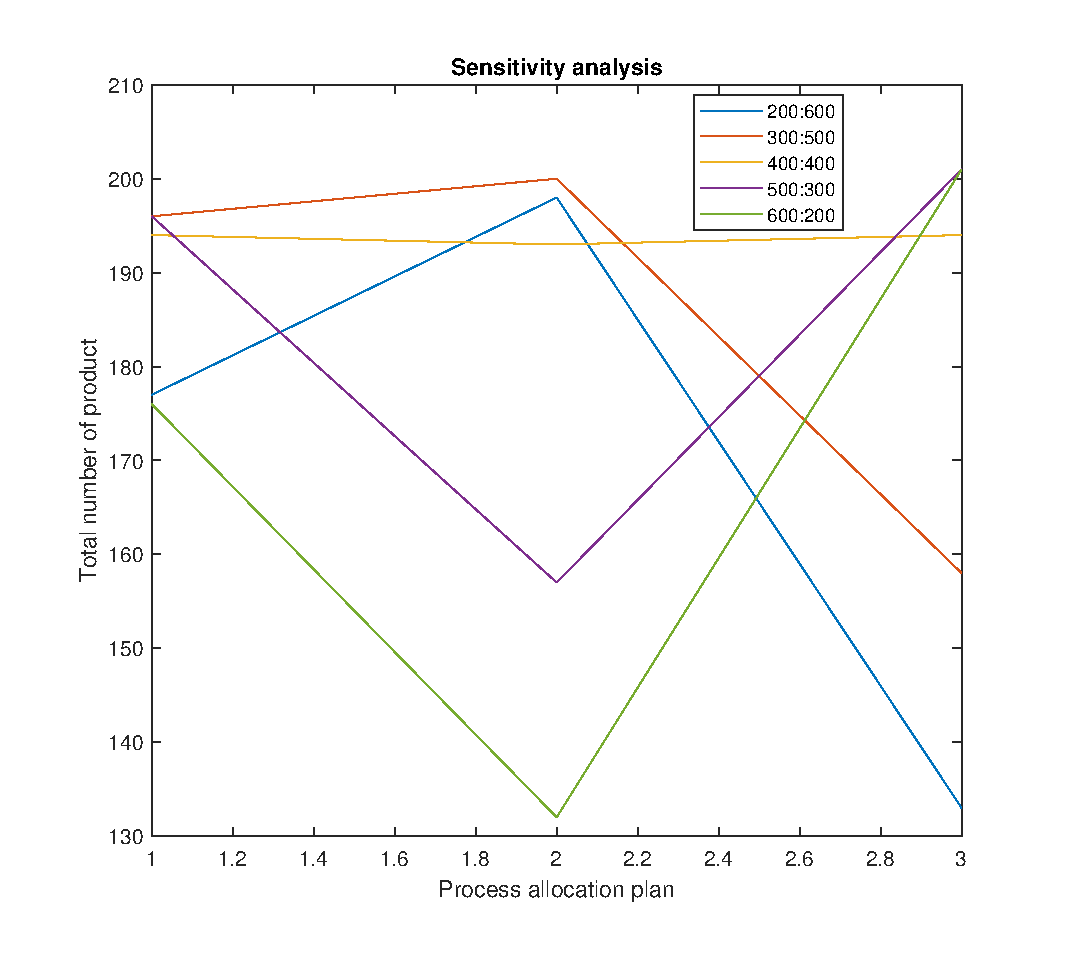
\includegraphics[width=0.7\textwidth]{sensitivity.eps}
	\caption{灵敏度分析}
     \label{figsen}
\end{figure}

\newpage
%参考文献
\begin{thebibliography}{9}%宽度9
\bibitem{bib1} 谢林江, 季桂树, 彭清, 等. 改进的卷积神经网络在行人检测中的应用[J].  计算机科学与探索,  2018,  12(5):708-718.
\bibitem{bib2}王耀玮, 唐伦, 刘云龙, 等. 基于多任务卷积神经网络的车辆多属性识别[J].  计算机工程与应用, 2018, 54(8):21-27.
\bibitem{bib3} Lenz I, Lee H, Saxena A. Deep learning for detecting robotic grasps[J]. The International Journal of Robotics Research, 2015, 34(4-5):705-724.
\bibitem{bib4} Kumra S, Kanan C. Robotic grasp detection using deep convolutional neural networks[C]//2017 IEEE/RSJ International Conference on Intelligent Robots and Systems (IROS). IEEE, 2017: 769-776.
\bibitem{bib5} Chu F J, Xu R, Vela P A. Real-world multiobject, multigrasp detection[J]. IEEE Robotics and Automation Letters, 2018, 3(4): 3355-3362.
\bibitem{bib6}  Robot Learning Lab: Learning to Grasp[EB/OL].(2009) [2019-03-12].
\bibitem{bib7}  Redmon J, Angelova A. Real-time grasp detection using convolutional neural networks[C]//2015 IEEE International Conference on Robotics and Automation (ICRA). IEEE, 2015: 1316-1322.
\bibitem{bib8} Ni P, Zhang W, Bai W, et al. A New Approach Based on Two-stream CNNs for Novel Objects Grasping in Clutter[J]. Journal of Intelligent \& Robotic Systems, 2018(2):1-17.
\bibitem{bib9} Krizhevsky A, Sutskever I, Hinton G E. Imagenet classification with deep convolutional neural networks[C]// Advances in neural information processing systems. 2012: 1097-1105.
\bibitem{bib10} He K, Zhang X, Ren S, et al. Deep residual learning for image recognition[C]//Proceedings of the IEEE conference on computer vision and pattern recognition. 2016: 770-778.
\bibitem{bib11} Qiang Z, Li Z, Li J, et al. Vehicle color recognition using
Multiple-Layer Feature Representations of lightweight convolutional neural network[J]. Signal Processing, 2018, 147: 146-153. 

\bibitem{bibb1} Dogar M, Hsiao K, Ciocarlie M, et al. Physics-based grasp planning through clutter[C]//Robotics: Science and Systems VIII. Cambridge, USA: MIT Press, 2012: 8pp.
\bibitem{bibb2} Goldfeder C, Ciocarlie M, Dang H, et al. The Columbia grasp database[C]//IEEE International Conference on Robotics and Automation. Piscataway, USA: IEEE, 2009: 1710-1716.
\bibitem{bibb3} Weisz J, Allen P K. Pose error robust grasping from contact wrench space metrics[C]//IEEE International Conference on Robotics and Automation. Piscataway, USA: IEEE, 2012: 557- 562.
\bibitem{bibb4}   Jiang Y, Moseson S, Saxena A. Efficient grasping from RGB-D images: Learning using a new rectangle representation[C]// IEEE International Conference on Robotics and Automation. Piscataway, USA: IEEE,2011: 3304-3311.
\bibitem{bibb5}  Hinton G E, Salakhutdinov R R. Reducing the dimensionality of data with neural networks[J]. Science, 2006, 313(5786): 504-507.
\bibitem{bibb6}   仲训杲,徐敏,仲训昱,等.基于多模特征深度学习的机器人抓取判别方法 [J].自动化学报,2016,42(7):1022- 1029.
\bibitem{bibb7} Lenz I, Lee H, Saxena A. Deep learning for detecting robotic grasps[J]. International Journal of Robotics Research, 2015, 34(4/5): 705-724.
\bibitem{bibb8}   杜学丹,蔡莹皓,鲁涛,等.一种基于深度学习的机械臂抓取方法  [J].机器人,2017,39(6):820-828,837.
\bibitem{bibb9} Pinto L, Gupta A. Supersizing self-supervision: Learning to grasp from 50k tries and 700 robot hours[C]//IEEE International Conference on Robotics and Automation. Piscataway, USA: IEEE, 2016: 3406-3413.
\bibitem{bibb10} Guo D, Sun F C, Liu H P, et al. A hybrid deep architecture for robotic grasp detection[C]//IEEE International Conference on Robotics and Automation. Piscataway, USA: IEEE, 2017: 1609-1614.
\bibitem{bibb11} 刘义军.基于 FPGA 的线结构光视觉测量系统研究 [D]. 长 春:吉林大学,2017:23-49.
\bibitem{bibb12} 邹媛媛,赵明扬,张雷.基于量块的线结构光视觉传感器直接标定方法 [J]. 中国激光,2014,41(11):189-194.
\bibitem{bibb13} 卢津,孙惠斌,常智勇.新型正交消隐点的摄像机标定方法 [J]. 中国激光,2014,41(2):294-302.

\bibitem{bibc1} 焦李成.神经网络系统理论[M].西安:西安电子科技大学出版社,1991.
\bibitem{bibc2} 何玉彬,李新忠.神经网络控制及其应用[M].北京:科学出版社,2000.
\bibitem{bibc3} McCulloch W S, Pitts W A. A logical calculus of the ideas immanent in nervous activity[J]. Bulletin of Mathematical Biophysics, 1943, 5: 115-133.
\bibitem{bibc4} Hebb D O. The Organization of Behaviour [M]. New York, John Wiley\&Sons Inc., 1949.
\bibitem{bibc5} Rosenblatt. The perception: a probabilistic model for information storage and organization in the brain [J]. Psychology Review, 1958, 65: 386-408.
\bibitem{bibc6} Minsky M, Papert S. Perceptron [M]. Cambridge, MA: MIT Press, 1969.
\bibitem{bibc7} Hopfield  J  J.  Neural  networks  and  physical  systems  with  emergent  collective computational  abilities[C].  Proceeding  of the National Academy  of  Science.  USA (Biophysics), 1982, 79: 2554-2558.
\bibitem{bibc8} Hopfield J J. Neurons with graded response have collective computational properties like those  of  two-state  neurons[C].  Proceedins  of  the  National  Academy  of  Science, USA(Biophysics), 1984, 81:3088-3092.
\bibitem{bibc9} Widrow B, McCool J, Ball M. The complex LMS algorithm [C]. Proc. IEEE, 1975, 63(4):719-720
\bibitem{bibc10} Hirose  A.  Complex-valued  neural  networks:  theories  and  applications  [M].  World Scientific Series on Innovation Intelligence, vol 5, Singapore: World Scientific Publishing Co. Pte. Ltd. 2003



 \bibitem{bib:one} 马倩倩,李晓娟,施智平.轻量级卷积神经网络的机器人抓取检测研究[J/OL].计算机工程与应用:1-11[2019-04-09].
 \bibitem{bib:two} 李传浩. 基于卷积神经网络的机器人自动抓取规划研究[D].哈尔滨工业大学,2018.
 \bibitem{bib:three} 夏晶,钱堃,马旭东,刘环.基于级联卷积神经网络的机器人平面抓取位姿快速检测[J].机器人,2018,40(06):794-802.
 \bibitem{bib:four} 胡琳,晁飞.基于双神经网络结构的发展型机器人3D抓取[J].电脑知识与技术,2012,8(12):2859-2862.
\bibitem{bib:five} 刘晓玉. 复杂环境下基于神经网络的工件识别与机器人智能抓取[D].武汉科技大学,2009.
\bibitem{bib:six} 游辉胜. 基于模糊神经网络的单目视觉伺服机器人智能抓取[D].武汉科技大学,2008.
\end{thebibliography}

\end{document} 